\documentclass[11pt]{article}

    \usepackage[T2A]{fontenc}
\usepackage[utf8]{inputenc}
\usepackage[english, russian]{babel}

\usepackage[breakable]{tcolorbox}
    \usepackage{parskip} % Stop auto-indenting (to mimic markdown behaviour)
    
    \usepackage{iftex}
    \ifPDFTeX
    	\usepackage[T1]{fontenc}
    	\usepackage{mathpazo}
    \else
    	\usepackage{fontspec}
    \fi

    % Basic figure setup, for now with no caption control since it's done
    % automatically by Pandoc (which extracts ![](path) syntax from Markdown).
    \usepackage{graphicx}
    % Maintain compatibility with old templates. Remove in nbconvert 6.0
    \let\Oldincludegraphics\includegraphics
    % Ensure that by default, figures have no caption (until we provide a
    % proper Figure object with a Caption API and a way to capture that
    % in the conversion process - todo).
    \usepackage{caption}
    \DeclareCaptionFormat{nocaption}{}
    \captionsetup{format=nocaption,aboveskip=0pt,belowskip=0pt}

    \usepackage{float}
    \floatplacement{figure}{H} % forces figures to be placed at the correct location
    \usepackage{xcolor} % Allow colors to be defined
    \usepackage{enumerate} % Needed for markdown enumerations to work
    \usepackage{geometry} % Used to adjust the document margins
    \usepackage{amsmath} % Equations
    \usepackage{amssymb} % Equations
    \usepackage{textcomp} % defines textquotesingle
    % Hack from http://tex.stackexchange.com/a/47451/13684:
    \AtBeginDocument{%
        \def\PYZsq{\textquotesingle}% Upright quotes in Pygmentized code
    }
    \usepackage{upquote} % Upright quotes for verbatim code
    \usepackage{eurosym} % defines \euro
    \usepackage[mathletters]{ucs} % Extended unicode (utf-8) support
    \usepackage{fancyvrb} % verbatim replacement that allows latex
    \usepackage{grffile} % extends the file name processing of package graphics 
                         % to support a larger range
    \makeatletter % fix for old versions of grffile with XeLaTeX
    \@ifpackagelater{grffile}{2019/11/01}
    {
      % Do nothing on new versions
    }
    {
      \def\Gread@@xetex#1{%
        \IfFileExists{"\Gin@base".bb}%
        {\Gread@eps{\Gin@base.bb}}%
        {\Gread@@xetex@aux#1}%
      }
    }
    \makeatother
    \usepackage[Export]{adjustbox} % Used to constrain images to a maximum size
    \adjustboxset{max size={0.9\linewidth}{0.9\paperheight}}

    % The hyperref package gives us a pdf with properly built
    % internal navigation ('pdf bookmarks' for the table of contents,
    % internal cross-reference links, web links for URLs, etc.)
    \usepackage{hyperref}
    % The default LaTeX title has an obnoxious amount of whitespace. By default,
    % titling removes some of it. It also provides customization options.
    \usepackage{titling}
    \usepackage{longtable} % longtable support required by pandoc >1.10
    \usepackage{booktabs}  % table support for pandoc > 1.12.2
    \usepackage[inline]{enumitem} % IRkernel/repr support (it uses the enumerate* environment)
    \usepackage[normalem]{ulem} % ulem is needed to support strikethroughs (\sout)
                                % normalem makes italics be italics, not underlines
    \usepackage{mathrsfs}
    
\usepackage{wrapfig}
\usepackage[rightcaption]{sidecap}
\providecommand{\keywords}[1]{\textbf{\textit{Keywords:}} #1}

\author{A. Yu. Drozdov}

    
    % Colors for the hyperref package
    \definecolor{urlcolor}{rgb}{0,.145,.698}
    \definecolor{linkcolor}{rgb}{.71,0.21,0.01}
    \definecolor{citecolor}{rgb}{.12,.54,.11}

    % ANSI colors
    \definecolor{ansi-black}{HTML}{3E424D}
    \definecolor{ansi-black-intense}{HTML}{282C36}
    \definecolor{ansi-red}{HTML}{E75C58}
    \definecolor{ansi-red-intense}{HTML}{B22B31}
    \definecolor{ansi-green}{HTML}{00A250}
    \definecolor{ansi-green-intense}{HTML}{007427}
    \definecolor{ansi-yellow}{HTML}{DDB62B}
    \definecolor{ansi-yellow-intense}{HTML}{B27D12}
    \definecolor{ansi-blue}{HTML}{208FFB}
    \definecolor{ansi-blue-intense}{HTML}{0065CA}
    \definecolor{ansi-magenta}{HTML}{D160C4}
    \definecolor{ansi-magenta-intense}{HTML}{A03196}
    \definecolor{ansi-cyan}{HTML}{60C6C8}
    \definecolor{ansi-cyan-intense}{HTML}{258F8F}
    \definecolor{ansi-white}{HTML}{C5C1B4}
    \definecolor{ansi-white-intense}{HTML}{A1A6B2}
    \definecolor{ansi-default-inverse-fg}{HTML}{FFFFFF}
    \definecolor{ansi-default-inverse-bg}{HTML}{000000}

    % common color for the border for error outputs.
    \definecolor{outerrorbackground}{HTML}{FFDFDF}

    % commands and environments needed by pandoc snippets
    % extracted from the output of `pandoc -s`
    \providecommand{\tightlist}{%
      \setlength{\itemsep}{0pt}\setlength{\parskip}{0pt}}
    \DefineVerbatimEnvironment{Highlighting}{Verbatim}{commandchars=\\\{\}}
    % Add ',fontsize=\small' for more characters per line
    \newenvironment{Shaded}{}{}
    \newcommand{\KeywordTok}[1]{\textcolor[rgb]{0.00,0.44,0.13}{\textbf{{#1}}}}
    \newcommand{\DataTypeTok}[1]{\textcolor[rgb]{0.56,0.13,0.00}{{#1}}}
    \newcommand{\DecValTok}[1]{\textcolor[rgb]{0.25,0.63,0.44}{{#1}}}
    \newcommand{\BaseNTok}[1]{\textcolor[rgb]{0.25,0.63,0.44}{{#1}}}
    \newcommand{\FloatTok}[1]{\textcolor[rgb]{0.25,0.63,0.44}{{#1}}}
    \newcommand{\CharTok}[1]{\textcolor[rgb]{0.25,0.44,0.63}{{#1}}}
    \newcommand{\StringTok}[1]{\textcolor[rgb]{0.25,0.44,0.63}{{#1}}}
    \newcommand{\CommentTok}[1]{\textcolor[rgb]{0.38,0.63,0.69}{\textit{{#1}}}}
    \newcommand{\OtherTok}[1]{\textcolor[rgb]{0.00,0.44,0.13}{{#1}}}
    \newcommand{\AlertTok}[1]{\textcolor[rgb]{1.00,0.00,0.00}{\textbf{{#1}}}}
    \newcommand{\FunctionTok}[1]{\textcolor[rgb]{0.02,0.16,0.49}{{#1}}}
    \newcommand{\RegionMarkerTok}[1]{{#1}}
    \newcommand{\ErrorTok}[1]{\textcolor[rgb]{1.00,0.00,0.00}{\textbf{{#1}}}}
    \newcommand{\NormalTok}[1]{{#1}}
    
    % Additional commands for more recent versions of Pandoc
    \newcommand{\ConstantTok}[1]{\textcolor[rgb]{0.53,0.00,0.00}{{#1}}}
    \newcommand{\SpecialCharTok}[1]{\textcolor[rgb]{0.25,0.44,0.63}{{#1}}}
    \newcommand{\VerbatimStringTok}[1]{\textcolor[rgb]{0.25,0.44,0.63}{{#1}}}
    \newcommand{\SpecialStringTok}[1]{\textcolor[rgb]{0.73,0.40,0.53}{{#1}}}
    \newcommand{\ImportTok}[1]{{#1}}
    \newcommand{\DocumentationTok}[1]{\textcolor[rgb]{0.73,0.13,0.13}{\textit{{#1}}}}
    \newcommand{\AnnotationTok}[1]{\textcolor[rgb]{0.38,0.63,0.69}{\textbf{\textit{{#1}}}}}
    \newcommand{\CommentVarTok}[1]{\textcolor[rgb]{0.38,0.63,0.69}{\textbf{\textit{{#1}}}}}
    \newcommand{\VariableTok}[1]{\textcolor[rgb]{0.10,0.09,0.49}{{#1}}}
    \newcommand{\ControlFlowTok}[1]{\textcolor[rgb]{0.00,0.44,0.13}{\textbf{{#1}}}}
    \newcommand{\OperatorTok}[1]{\textcolor[rgb]{0.40,0.40,0.40}{{#1}}}
    \newcommand{\BuiltInTok}[1]{{#1}}
    \newcommand{\ExtensionTok}[1]{{#1}}
    \newcommand{\PreprocessorTok}[1]{\textcolor[rgb]{0.74,0.48,0.00}{{#1}}}
    \newcommand{\AttributeTok}[1]{\textcolor[rgb]{0.49,0.56,0.16}{{#1}}}
    \newcommand{\InformationTok}[1]{\textcolor[rgb]{0.38,0.63,0.69}{\textbf{\textit{{#1}}}}}
    \newcommand{\WarningTok}[1]{\textcolor[rgb]{0.38,0.63,0.69}{\textbf{\textit{{#1}}}}}
    
    
    % Define a nice break command that doesn't care if a line doesn't already
    % exist.
    \def\br{\hspace*{\fill} \\* }
    % Math Jax compatibility definitions
    \def\gt{>}
    \def\lt{<}
    \let\Oldtex\TeX
    \let\Oldlatex\LaTeX
    \renewcommand{\TeX}{\textrm{\Oldtex}}
    \renewcommand{\LaTeX}{\textrm{\Oldlatex}}
    % Document parameters
    % Document title
    \title{Fermi1923}
    
    
    
    
    
% Pygments definitions
\makeatletter
\def\PY@reset{\let\PY@it=\relax \let\PY@bf=\relax%
    \let\PY@ul=\relax \let\PY@tc=\relax%
    \let\PY@bc=\relax \let\PY@ff=\relax}
\def\PY@tok#1{\csname PY@tok@#1\endcsname}
\def\PY@toks#1+{\ifx\relax#1\empty\else%
    \PY@tok{#1}\expandafter\PY@toks\fi}
\def\PY@do#1{\PY@bc{\PY@tc{\PY@ul{%
    \PY@it{\PY@bf{\PY@ff{#1}}}}}}}
\def\PY#1#2{\PY@reset\PY@toks#1+\relax+\PY@do{#2}}

\@namedef{PY@tok@w}{\def\PY@tc##1{\textcolor[rgb]{0.73,0.73,0.73}{##1}}}
\@namedef{PY@tok@c}{\let\PY@it=\textit\def\PY@tc##1{\textcolor[rgb]{0.25,0.50,0.50}{##1}}}
\@namedef{PY@tok@cp}{\def\PY@tc##1{\textcolor[rgb]{0.74,0.48,0.00}{##1}}}
\@namedef{PY@tok@k}{\let\PY@bf=\textbf\def\PY@tc##1{\textcolor[rgb]{0.00,0.50,0.00}{##1}}}
\@namedef{PY@tok@kp}{\def\PY@tc##1{\textcolor[rgb]{0.00,0.50,0.00}{##1}}}
\@namedef{PY@tok@kt}{\def\PY@tc##1{\textcolor[rgb]{0.69,0.00,0.25}{##1}}}
\@namedef{PY@tok@o}{\def\PY@tc##1{\textcolor[rgb]{0.40,0.40,0.40}{##1}}}
\@namedef{PY@tok@ow}{\let\PY@bf=\textbf\def\PY@tc##1{\textcolor[rgb]{0.67,0.13,1.00}{##1}}}
\@namedef{PY@tok@nb}{\def\PY@tc##1{\textcolor[rgb]{0.00,0.50,0.00}{##1}}}
\@namedef{PY@tok@nf}{\def\PY@tc##1{\textcolor[rgb]{0.00,0.00,1.00}{##1}}}
\@namedef{PY@tok@nc}{\let\PY@bf=\textbf\def\PY@tc##1{\textcolor[rgb]{0.00,0.00,1.00}{##1}}}
\@namedef{PY@tok@nn}{\let\PY@bf=\textbf\def\PY@tc##1{\textcolor[rgb]{0.00,0.00,1.00}{##1}}}
\@namedef{PY@tok@ne}{\let\PY@bf=\textbf\def\PY@tc##1{\textcolor[rgb]{0.82,0.25,0.23}{##1}}}
\@namedef{PY@tok@nv}{\def\PY@tc##1{\textcolor[rgb]{0.10,0.09,0.49}{##1}}}
\@namedef{PY@tok@no}{\def\PY@tc##1{\textcolor[rgb]{0.53,0.00,0.00}{##1}}}
\@namedef{PY@tok@nl}{\def\PY@tc##1{\textcolor[rgb]{0.63,0.63,0.00}{##1}}}
\@namedef{PY@tok@ni}{\let\PY@bf=\textbf\def\PY@tc##1{\textcolor[rgb]{0.60,0.60,0.60}{##1}}}
\@namedef{PY@tok@na}{\def\PY@tc##1{\textcolor[rgb]{0.49,0.56,0.16}{##1}}}
\@namedef{PY@tok@nt}{\let\PY@bf=\textbf\def\PY@tc##1{\textcolor[rgb]{0.00,0.50,0.00}{##1}}}
\@namedef{PY@tok@nd}{\def\PY@tc##1{\textcolor[rgb]{0.67,0.13,1.00}{##1}}}
\@namedef{PY@tok@s}{\def\PY@tc##1{\textcolor[rgb]{0.73,0.13,0.13}{##1}}}
\@namedef{PY@tok@sd}{\let\PY@it=\textit\def\PY@tc##1{\textcolor[rgb]{0.73,0.13,0.13}{##1}}}
\@namedef{PY@tok@si}{\let\PY@bf=\textbf\def\PY@tc##1{\textcolor[rgb]{0.73,0.40,0.53}{##1}}}
\@namedef{PY@tok@se}{\let\PY@bf=\textbf\def\PY@tc##1{\textcolor[rgb]{0.73,0.40,0.13}{##1}}}
\@namedef{PY@tok@sr}{\def\PY@tc##1{\textcolor[rgb]{0.73,0.40,0.53}{##1}}}
\@namedef{PY@tok@ss}{\def\PY@tc##1{\textcolor[rgb]{0.10,0.09,0.49}{##1}}}
\@namedef{PY@tok@sx}{\def\PY@tc##1{\textcolor[rgb]{0.00,0.50,0.00}{##1}}}
\@namedef{PY@tok@m}{\def\PY@tc##1{\textcolor[rgb]{0.40,0.40,0.40}{##1}}}
\@namedef{PY@tok@gh}{\let\PY@bf=\textbf\def\PY@tc##1{\textcolor[rgb]{0.00,0.00,0.50}{##1}}}
\@namedef{PY@tok@gu}{\let\PY@bf=\textbf\def\PY@tc##1{\textcolor[rgb]{0.50,0.00,0.50}{##1}}}
\@namedef{PY@tok@gd}{\def\PY@tc##1{\textcolor[rgb]{0.63,0.00,0.00}{##1}}}
\@namedef{PY@tok@gi}{\def\PY@tc##1{\textcolor[rgb]{0.00,0.63,0.00}{##1}}}
\@namedef{PY@tok@gr}{\def\PY@tc##1{\textcolor[rgb]{1.00,0.00,0.00}{##1}}}
\@namedef{PY@tok@ge}{\let\PY@it=\textit}
\@namedef{PY@tok@gs}{\let\PY@bf=\textbf}
\@namedef{PY@tok@gp}{\let\PY@bf=\textbf\def\PY@tc##1{\textcolor[rgb]{0.00,0.00,0.50}{##1}}}
\@namedef{PY@tok@go}{\def\PY@tc##1{\textcolor[rgb]{0.53,0.53,0.53}{##1}}}
\@namedef{PY@tok@gt}{\def\PY@tc##1{\textcolor[rgb]{0.00,0.27,0.87}{##1}}}
\@namedef{PY@tok@err}{\def\PY@bc##1{{\setlength{\fboxsep}{\string -\fboxrule}\fcolorbox[rgb]{1.00,0.00,0.00}{1,1,1}{\strut ##1}}}}
\@namedef{PY@tok@kc}{\let\PY@bf=\textbf\def\PY@tc##1{\textcolor[rgb]{0.00,0.50,0.00}{##1}}}
\@namedef{PY@tok@kd}{\let\PY@bf=\textbf\def\PY@tc##1{\textcolor[rgb]{0.00,0.50,0.00}{##1}}}
\@namedef{PY@tok@kn}{\let\PY@bf=\textbf\def\PY@tc##1{\textcolor[rgb]{0.00,0.50,0.00}{##1}}}
\@namedef{PY@tok@kr}{\let\PY@bf=\textbf\def\PY@tc##1{\textcolor[rgb]{0.00,0.50,0.00}{##1}}}
\@namedef{PY@tok@bp}{\def\PY@tc##1{\textcolor[rgb]{0.00,0.50,0.00}{##1}}}
\@namedef{PY@tok@fm}{\def\PY@tc##1{\textcolor[rgb]{0.00,0.00,1.00}{##1}}}
\@namedef{PY@tok@vc}{\def\PY@tc##1{\textcolor[rgb]{0.10,0.09,0.49}{##1}}}
\@namedef{PY@tok@vg}{\def\PY@tc##1{\textcolor[rgb]{0.10,0.09,0.49}{##1}}}
\@namedef{PY@tok@vi}{\def\PY@tc##1{\textcolor[rgb]{0.10,0.09,0.49}{##1}}}
\@namedef{PY@tok@vm}{\def\PY@tc##1{\textcolor[rgb]{0.10,0.09,0.49}{##1}}}
\@namedef{PY@tok@sa}{\def\PY@tc##1{\textcolor[rgb]{0.73,0.13,0.13}{##1}}}
\@namedef{PY@tok@sb}{\def\PY@tc##1{\textcolor[rgb]{0.73,0.13,0.13}{##1}}}
\@namedef{PY@tok@sc}{\def\PY@tc##1{\textcolor[rgb]{0.73,0.13,0.13}{##1}}}
\@namedef{PY@tok@dl}{\def\PY@tc##1{\textcolor[rgb]{0.73,0.13,0.13}{##1}}}
\@namedef{PY@tok@s2}{\def\PY@tc##1{\textcolor[rgb]{0.73,0.13,0.13}{##1}}}
\@namedef{PY@tok@sh}{\def\PY@tc##1{\textcolor[rgb]{0.73,0.13,0.13}{##1}}}
\@namedef{PY@tok@s1}{\def\PY@tc##1{\textcolor[rgb]{0.73,0.13,0.13}{##1}}}
\@namedef{PY@tok@mb}{\def\PY@tc##1{\textcolor[rgb]{0.40,0.40,0.40}{##1}}}
\@namedef{PY@tok@mf}{\def\PY@tc##1{\textcolor[rgb]{0.40,0.40,0.40}{##1}}}
\@namedef{PY@tok@mh}{\def\PY@tc##1{\textcolor[rgb]{0.40,0.40,0.40}{##1}}}
\@namedef{PY@tok@mi}{\def\PY@tc##1{\textcolor[rgb]{0.40,0.40,0.40}{##1}}}
\@namedef{PY@tok@il}{\def\PY@tc##1{\textcolor[rgb]{0.40,0.40,0.40}{##1}}}
\@namedef{PY@tok@mo}{\def\PY@tc##1{\textcolor[rgb]{0.40,0.40,0.40}{##1}}}
\@namedef{PY@tok@ch}{\let\PY@it=\textit\def\PY@tc##1{\textcolor[rgb]{0.25,0.50,0.50}{##1}}}
\@namedef{PY@tok@cm}{\let\PY@it=\textit\def\PY@tc##1{\textcolor[rgb]{0.25,0.50,0.50}{##1}}}
\@namedef{PY@tok@cpf}{\let\PY@it=\textit\def\PY@tc##1{\textcolor[rgb]{0.25,0.50,0.50}{##1}}}
\@namedef{PY@tok@c1}{\let\PY@it=\textit\def\PY@tc##1{\textcolor[rgb]{0.25,0.50,0.50}{##1}}}
\@namedef{PY@tok@cs}{\let\PY@it=\textit\def\PY@tc##1{\textcolor[rgb]{0.25,0.50,0.50}{##1}}}

\def\PYZbs{\char`\\}
\def\PYZus{\char`\_}
\def\PYZob{\char`\{}
\def\PYZcb{\char`\}}
\def\PYZca{\char`\^}
\def\PYZam{\char`\&}
\def\PYZlt{\char`\<}
\def\PYZgt{\char`\>}
\def\PYZsh{\char`\#}
\def\PYZpc{\char`\%}
\def\PYZdl{\char`\$}
\def\PYZhy{\char`\-}
\def\PYZsq{\char`\'}
\def\PYZdq{\char`\"}
\def\PYZti{\char`\~}
% for compatibility with earlier versions
\def\PYZat{@}
\def\PYZlb{[}
\def\PYZrb{]}
\makeatother


    % For linebreaks inside Verbatim environment from package fancyvrb. 
    \makeatletter
        \newbox\Wrappedcontinuationbox 
        \newbox\Wrappedvisiblespacebox 
        \newcommand*\Wrappedvisiblespace {\textcolor{red}{\textvisiblespace}} 
        \newcommand*\Wrappedcontinuationsymbol {\textcolor{red}{\llap{\tiny$\m@th\hookrightarrow$}}} 
        \newcommand*\Wrappedcontinuationindent {3ex } 
        \newcommand*\Wrappedafterbreak {\kern\Wrappedcontinuationindent\copy\Wrappedcontinuationbox} 
        % Take advantage of the already applied Pygments mark-up to insert 
        % potential linebreaks for TeX processing. 
        %        {, <, #, %, $, ' and ": go to next line. 
        %        _, }, ^, &, >, - and ~: stay at end of broken line. 
        % Use of \textquotesingle for straight quote. 
        \newcommand*\Wrappedbreaksatspecials {% 
            \def\PYGZus{\discretionary{\char`\_}{\Wrappedafterbreak}{\char`\_}}% 
            \def\PYGZob{\discretionary{}{\Wrappedafterbreak\char`\{}{\char`\{}}% 
            \def\PYGZcb{\discretionary{\char`\}}{\Wrappedafterbreak}{\char`\}}}% 
            \def\PYGZca{\discretionary{\char`\^}{\Wrappedafterbreak}{\char`\^}}% 
            \def\PYGZam{\discretionary{\char`\&}{\Wrappedafterbreak}{\char`\&}}% 
            \def\PYGZlt{\discretionary{}{\Wrappedafterbreak\char`\<}{\char`\<}}% 
            \def\PYGZgt{\discretionary{\char`\>}{\Wrappedafterbreak}{\char`\>}}% 
            \def\PYGZsh{\discretionary{}{\Wrappedafterbreak\char`\#}{\char`\#}}% 
            \def\PYGZpc{\discretionary{}{\Wrappedafterbreak\char`\%}{\char`\%}}% 
            \def\PYGZdl{\discretionary{}{\Wrappedafterbreak\char`\$}{\char`\$}}% 
            \def\PYGZhy{\discretionary{\char`\-}{\Wrappedafterbreak}{\char`\-}}% 
            \def\PYGZsq{\discretionary{}{\Wrappedafterbreak\textquotesingle}{\textquotesingle}}% 
            \def\PYGZdq{\discretionary{}{\Wrappedafterbreak\char`\"}{\char`\"}}% 
            \def\PYGZti{\discretionary{\char`\~}{\Wrappedafterbreak}{\char`\~}}% 
        } 
        % Some characters . , ; ? ! / are not pygmentized. 
        % This macro makes them "active" and they will insert potential linebreaks 
        \newcommand*\Wrappedbreaksatpunct {% 
            \lccode`\~`\.\lowercase{\def~}{\discretionary{\hbox{\char`\.}}{\Wrappedafterbreak}{\hbox{\char`\.}}}% 
            \lccode`\~`\,\lowercase{\def~}{\discretionary{\hbox{\char`\,}}{\Wrappedafterbreak}{\hbox{\char`\,}}}% 
            \lccode`\~`\;\lowercase{\def~}{\discretionary{\hbox{\char`\;}}{\Wrappedafterbreak}{\hbox{\char`\;}}}% 
            \lccode`\~`\:\lowercase{\def~}{\discretionary{\hbox{\char`\:}}{\Wrappedafterbreak}{\hbox{\char`\:}}}% 
            \lccode`\~`\?\lowercase{\def~}{\discretionary{\hbox{\char`\?}}{\Wrappedafterbreak}{\hbox{\char`\?}}}% 
            \lccode`\~`\!\lowercase{\def~}{\discretionary{\hbox{\char`\!}}{\Wrappedafterbreak}{\hbox{\char`\!}}}% 
            \lccode`\~`\/\lowercase{\def~}{\discretionary{\hbox{\char`\/}}{\Wrappedafterbreak}{\hbox{\char`\/}}}% 
            \catcode`\.\active
            \catcode`\,\active 
            \catcode`\;\active
            \catcode`\:\active
            \catcode`\?\active
            \catcode`\!\active
            \catcode`\/\active 
            \lccode`\~`\~ 	
        }
    \makeatother

    \let\OriginalVerbatim=\Verbatim
    \makeatletter
    \renewcommand{\Verbatim}[1][1]{%
        %\parskip\z@skip
        \sbox\Wrappedcontinuationbox {\Wrappedcontinuationsymbol}%
        \sbox\Wrappedvisiblespacebox {\FV@SetupFont\Wrappedvisiblespace}%
        \def\FancyVerbFormatLine ##1{\hsize\linewidth
            \vtop{\raggedright\hyphenpenalty\z@\exhyphenpenalty\z@
                \doublehyphendemerits\z@\finalhyphendemerits\z@
                \strut ##1\strut}%
        }%
        % If the linebreak is at a space, the latter will be displayed as visible
        % space at end of first line, and a continuation symbol starts next line.
        % Stretch/shrink are however usually zero for typewriter font.
        \def\FV@Space {%
            \nobreak\hskip\z@ plus\fontdimen3\font minus\fontdimen4\font
            \discretionary{\copy\Wrappedvisiblespacebox}{\Wrappedafterbreak}
            {\kern\fontdimen2\font}%
        }%
        
        % Allow breaks at special characters using \PYG... macros.
        \Wrappedbreaksatspecials
        % Breaks at punctuation characters . , ; ? ! and / need catcode=\active 	
        \OriginalVerbatim[#1,codes*=\Wrappedbreaksatpunct]%
    }
    \makeatother

    % Exact colors from NB
    \definecolor{incolor}{HTML}{303F9F}
    \definecolor{outcolor}{HTML}{D84315}
    \definecolor{cellborder}{HTML}{CFCFCF}
    \definecolor{cellbackground}{HTML}{F7F7F7}
    
    % prompt
    \makeatletter
    \newcommand{\boxspacing}{\kern\kvtcb@left@rule\kern\kvtcb@boxsep}
    \makeatother
    \newcommand{\prompt}[4]{
        {\ttfamily\llap{{\color{#2}[#3]:\hspace{3pt}#4}}\vspace{-\baselineskip}}
    }
    

    
    % Prevent overflowing lines due to hard-to-break entities
    \sloppy 
    % Setup hyperref package
    \hypersetup{
      breaklinks=true,  % so long urls are correctly broken across lines
      colorlinks=true,
      urlcolor=urlcolor,
      linkcolor=linkcolor,
      citecolor=citecolor,
      }
    % Slightly bigger margins than the latex defaults
    
    \geometry{verbose,tmargin=1in,bmargin=1in,lmargin=1in,rmargin=1in}
    
    

\begin{document}
    
    \maketitle
    
    

    
    Противоречие между теориями электромагнитной массы

    РАЗРЕШЕНИЕ СУЩЕСТВУЮЩЕГО ПРОТИВОРЕЧИЯ МЕЖДУ ЭЛЕКТРОДИНАМИЧЕСКОЙ И
РЕЛЯТИВИСТСКОЙ ТЕОРИЯМИ ЭЛЕКТРОМАГНИТНОЙ МАССЫ*\(^1\)

    *Correzione di una contraddizione tra la teoria elettrodinamica e quella
relativistica delle masse elettromagnetiche. Nuovo Cimento, 1923, 25,
159-170

    \(^1\) Относительно этого вопроса см. две работы: E. Fermi. Rend. Lincei
(5), 1922, 31, 184, 306. {[}Статья Б5б{]}.

    § 1. Теория электромагнитной массы впервые была развита М.
Абрагамом\(^2\) еще до открытия теории относительности. Поэтому Абрагам
в своих расчетах, естественно, рассматривал массу системы электрических
зарядов, жестко связанных между собой в смысле классической механики.

    \(^2\) A b r a g a m. Theorie der Elektricitat; R i c h a r d s o n.
Electron Theory of Matter, Chap. XI; L o r e n t z. The Theory of
Electrons, p. 37.

    Он нашел, что при сферической симметрии системы ее масса зависит от
скорости, причем для нулевых или очень малых скоростей она равна\(^3\)
\(\left(\frac{4}{3}\right) \frac{u}{c^2}\) (где \(u\) -
электростатическая энергия системы и \(c\) - скорость света). Для
скоростей же \(v\), сравнимых с \(c\), появляются довольно сложные
поправочные члены порядка \(\frac{v^2}{c^2}\). Еще до теории
относительности Фицджеральд ввел гипотезу о том, что твердые тела
испытывают сокращение в направлении их движения в отношении

\[\sqrt{1-\frac{v^2}{c^2}}:1\]

    и Лоренц переработал теорию электромагнитной массы Абрагама, рассмотрев
теперь системы, испытывающие это сокращение, а не системы электрических
зарядов, жестко связанных в смысле классической механики.

    \(^3\) Обычно говорят, что электромагнитная масса равномерно заряженного
сферического слоя с общим зарадом \(e\) и радиусом \(r\) равна
\(\frac{2}{3} \frac{e^2}{r c^2}\); если же заметить, что
электростатическая энергия \(u = \frac{1}{2} \frac{e^2}{r}\), то для
массы находим как раз \(\left(\frac{4}{3}\right) \frac{u}{c^2}\).

    Лоренц нашел, что масса покоя (т. е. предел массы для нулевых скоростей)
по-прежнему равна \(\left({}^{4}\big/{}_{3}\right) \, \frac{u}{c^2}\), а
поправочные члены, зависящие от \(\frac{v^2}{c^2}\), изменились.

    Опыты Кауфмана, Бухерера и других, иследоваших массу частиц
\(\alpha\)-радиоактивных тел и катодных частиц большой скорости,
определенно говорили в пользу так называемой теории «деформируемого»
электрона Лоренца и против теории «твердого» электрона Абрагама. Вначале
это интерпретировалось как доказательство исключительно электромагнитной
природы массы электрона, так как счигалось, что иначе их масса должна
была бы быть постоянна. Впоследствии появление теории относительности
привело к тому взгляду, что все массы как электромагнитной, так и другой
природы должны зависеть от скорости, равно как и масса деформируемого
электрона Лоренца. Таким образом, указанные опыты оставляли открытым
вопрос о том, полностью ли электромагнитна масса электрона, и
представляли собой лишь подтверждение теории относительности. С другой
стороны, специальная теория относительности, не говоря уже об общей
теории относительности, привела к необходимости приписать системе с
энергией \(u\) массу \(u/c^2\); итак, возникло серьезное разногласие
между электродинамической теорией Лоренца, которая приписывает
сферическому распределению электрического заряда массу покоя
\(\left({}^{4}\big/{}_{3}\right) \, u/c^2\), и теорией относительности,
согласно которой соответствующая масса равна \(u/c^2\). Такое
разногласие\(^4\) представляется особенно серьезным, если учесть большую
важность понятия электромагнитной массы как основы электронной теории
материи.

    \(^4\) Опыты Кауфмана и других, естественно, не помогают решению вопроса
о том, какой из двух результатов является правильным. На самом деле они
позволяют определить только зависящие от скорости поправочные члены,
которые одинаковы в обеих теориях (отличие же существует в значениях
масс покоя).

    Это разногласие показалось мне особенно острым в двух недавних
работах\(^5\), в одной из которых, рассматривая электромагнитные массы
систем с произвольной симметрией на основании обычных электромагнитных
теорий, я нашел, что вообще массы представляются не скалярами, а
тензорами, естественно переходящими в
\(\left({}^{4} \big /{}_{3}\right) \, u/c^2\) при сферической симметрии.
Исходя из общей теории относительности, в другой работе я рассмотрел вес
тех же самых систем и нашел его во всех случаях равным
\(\left(u/c^2\right)G\) (где \(G\) - гравитационное ускорение).

    \(^5\) E. Fermi. Nuovo Cimento, 1921, VI, 22, 176, 199. (Статьи 2 и 1.)

    В настоящей работе мы покажем, что различие значений массы, полученных
двумя способами, обусловлено противоречащим принципу относительности
понятием жесткости, которое используется в электродинамической теории
(даже в теории деформируемого электрона). Эта концепция приводит к массе
\(\left({}^{4} \big /{}_{3}\right) \, u/c^2\), в то время как более
обоснованное, согласующееся с теорией относительности понятие абсолютно
твердого тела приводит к значению \(u/c^2\).

    Заметим еще, что релятивистская динамика электрона была развита М.
Борном \(^6\), который, однако, воспользовавшись точкой зрения, по
существу не отличающейся от обычной, естественно, нашел для массы покоя
\(\left({}^{4} \big /{}_{3}\right) \, u/c^2\)

    \(^6\) M. Born. Ann. d. Phys., 1909, 30, 1.

    В наших рассуждениях мы берем за основу принцип Гамильтона как наиболее
удобный для решения задачи, в которой связи довольно сложны.
Действительно, наша система электрических зарядов должна иметь связи
совсем иного типа, чем связи, рассматриваемые в обычной механике
(вследствие принципа относительности система, в зависимости от своей
скорости, будет испытывать лоренцово сокращение). Однако, во избежание
недоразумений, сразу заметим, что хотя сокращение Лоренца имеет порядок
\({v^2} \big /{c^2}\), его влияние на электромагнитную массу касается ее
основных членов (т. е. массы покоя). Поэтому оно ощутимо даже при очень
низких скоростях.

    § 2. Итак, рассмотрим систему электрических зарядов, находящихся в
абсолютно твердом диэлектрике. Предположим, что под действием
электромагнитного поля, обусловленного частично самой системой, частично
же внешними причинами, система находится в состоянии поступательного
движения, описывая в пространстве-времени\(^7\) мировую трубку.

    \(^7\) Далее пространство - время считается эвклидовым, поскольку
подразумевается, что рассматриваемые электромагнитные поля недостаточно
сильны для того, чтобы заметно изменить его метрическую структуру.

    Сформулируем точно, что именно следует понимать под поступательным
движением абсолютно твердого тела. Для этого рассмотрим некоторую
систему отсчета Лоренца - Эйнштейна и предположим, что в данный момент
времени для нее одна точка системы зарядов имеет скорость, равную нулю;
мы будем называть движение поступательным, если для этого момента
времени в той же самой системе отсчета все точки нашей системы зарядов
имеют скорость, равную нулю. Это равносильно утверждению, что мировые
линии точек нашей системы суть трактории, ортогональные семейству
линейных пространств. И действительно, в системе отсчета Лоренца -
Эйнштейна, в которой пространство является одним из пространств
семейства и временная ось, естественно, перпендикулярна ему вся система
находится в покое в нулевой момент времени, поскольку пространство
ортогонально пересекает мировые линии всех точек системы. При таком
определении поступательного движения, по существу принятом М. Борном,
жесткость системы выражается тем фактом, что ее форма в этих
пространствах, перпендикулярных трубке остается неизменной т. е. все
нормальные сечения трубки равны друг другу.

    Чтобы применить к нашему случаю принцип Гамильтона, необходимо знать
вариацию движения нашей системы, удовлетворяющую связям данной задачи,
т. е. правильно интерпретируемой жесткости. Далее мы покажем, что для
электромагнитной массы получается значение
\(\left({}^{4} \big /{}_{3}\right) \, u/c^2\) или \(u/c^2\) в
зависимости от того, какая из двух ниже иллюстрируемых и обозначенных
буквами А и В) вариаций принимается. Сразу же будет видно, что вариацию
А не следует принимать во внимание, поскольку она противоречит принципу
относительности. Пусть Т - мировая трубка, описанная системой. На
рисунке пространство \((x, y, z)\) представлено только одним измерением
--- осью \(x\), и вместо времени \(t\) используется \(ict\), чтобы иметь
определенную метрику.

    Вариация А. В качестве вариации, удовлетворяющей жесткой связи,
рассматривается бесконечно малое смещение, жесткое в обычном
кинематическом смысле; это смещение каждого сечения трубки,
параллельного пространству \((x, y, z)\), является параллельным этому
пространству. Такую вариацию получим, смещая параллельно оси \(x\) (см.
рисунок) каждое сечение \(t = const\) трубки на произвольный бесконечно
малый отрезок. Если мы ограничимся трансляционными смещениями, то
\(\delta x, \delta y, \delta z\) --- произвольные функции только времени,
а \(\delta t = 0\).

    \begin{figure}
\centering
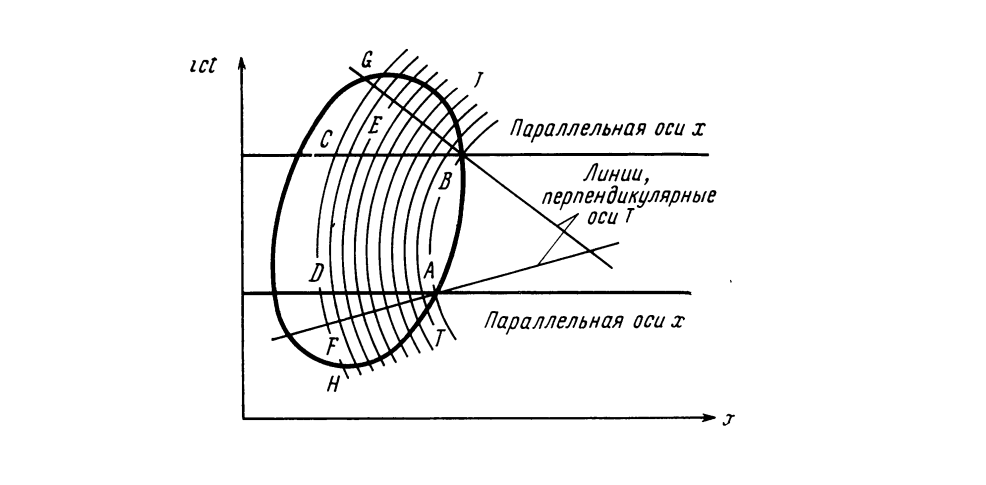
\includegraphics{Fermi1923.png}
\caption{Fermi1923.png}
\end{figure}

    Вариация В. В качестве вариации, удовлетворяющей жесткой связи
рассматривается бесконечно малое и жесткое в обычном кинематическом
смысле смещение каждого нормального сечения трубки, перпендикулярное
самой трубке. На рисунке такую вариацию получим, смещая каждое
нормальное сечение трубки параллельно самому себе на произвольный
отрезок.

    Из этих двух вариаций А явно противоречит принципу относительности; ее
можно не принимать во внимание, поскольку она даже неинвариантна
относительно преобразований Лоренца и на самом деле определяется самой
выбранной системой отсчета \((x, y, z)\); она никак не может быть
выражением физических понятий, таких, как понятие абсолютно твердого
тела. Напротив, вариация В явно удовлетворяет указанному условию
инвариантности; кроме того, поскольку она зависит только от элементов
трубки Т, полностью независимых от положения осей системы отсчега,
только она и будег естественной. Действительно, она основывается на
соотвегствующем понятию абсолютно твердого тела виртуальном смещении в
такой системе отсчета, по отношению к которой в рассматриваемый момент
времени скорость системы зарядов равна нулю. Поверхностно рассуждая,
можно было бы думать, что вариации А и В приводят к существенно
различным следствиям только при больших скоростях, т. е. когда трубка Т
составляет значительный угол с временной осью. Но расчеты, которые мы
будем развивать, сразу покажут, что разница существенна уже для нулевых
скоростей и что А дает для электромагнитной массы
\(\left({}^{4} \big /{}_{3}\right) \, u/c^2\), в то время как В дает
\(u/c^2\).

    § 3. Обозначим через \((t, x, y, z)\), или \((x_0, x_1, x_2, x_3)\),
координаты времени и пространства; при этом выбор обозначений
определяется только соображениями удобства. Пусть \(\varphi_i\) -
четырехмерный потенциал и

\[F_{ik}=\frac{\partial \varphi_i}{\partial x_k} - \frac{\partial \varphi_k}{\partial x_i}\]
- электромагнитное поле, а \(E\) и \(H\) - напряженности электрического
и магнитного полей, соотвествующие ему.

    Принцип Гамильтона, суммирующий законы Максвелла - Лоренца и законы
механики, гласит\(^8\), что суммарное действие, т. е. сумма действий
электромагнитного поля и «материальных» и электрических масс не меняется
в результате произвольной вариации \(\varphi_i\) и координат точек
мировых линий электрических зарядов, которая соответствует связям и
равна нулю на границе области интегрирования. В нашем случае
«материальных» масс нет, и единственные величины, которые подвергаются
варьированию, суть координаты точек мировых линий зарядов; поэтому
достаточно рассмотреть только действие электрических зарядов, т. е.

\[W=\sum_i\int de \int \varphi_i dx_i.\]

    Здесь \(de\) --- элемент электрического заряда, и второй интеграл должен
быть взят по такому отрезку описанной \(de\) мировой линии, который
находится внутри четырехмерной области \(G\) интегрирования. Поэтому для
каждой системы вариаций \(\delta {{x}_{і}}\), соответствующих связям и
обращающихся в нуль на границе \(G\), должно быть \(\delta W = 0\),

    т. е.

\[\sum_{ik} \int \int de F_{ik} \delta {{x}_{і}} dx_{k} = 0. \,\,\,(1)\]

    \(^8\) W e y l. Raum, Zeit, Materie. Berlin, Springer, 1921, p. 194-196.

    Теперь необходимо рассмотреть по отдельности результаты, которые
получаются при подстановке значений \(\delta {{x}_{і}}\), следующих из
вариаций типа А или В.

    4. Следствия вариаций типа А. В этом случае область интегрирование
сводится просто к ABCD. И действительно, области BCG, ADH не дают
никакого вклада, поскольку поскольку все \(\delta {{x}_{і}}\) в них равны
нулю; это происходит оттого, что на контуре \(G\), и поэтому на пути BG,
АН величины \(\delta {{x}_{і}}\) должны быть равны нулю, а для постоянного
\(t\), т. е. на линиях, параллельных оси \(x\), они должны иметь
постоянное значение. Если через \(t_1\) и \(t_2\) обозначить моменты
времени, соответствующие А и В, то выражение (1) можно записать
следующим образом:

\[\sum_{ik} \int\limits_{t_1}^{t_2} dt \delta {{x}_{і}} \int de F_{ik}  \frac{dx_{k}}{dt} \,\,\,(i = 1,2,3)\,\,\,(k = 0,1,2,3)\]

(\(\delta t = 0\), а \(\delta x\), \(\delta y\), \(\delta z\) ---
функции только времени). Поскольку \(\delta {{x}_{і}}\) - произвольные функции
\(t\), получим три уравнения

\[\int de \sum_{k} F_{ik}  \frac{dx_{k}}{dt} = 0\]

т. е.

\[\int de \, \left[ E_{x}  + \frac{dy}{dt} H_{z} - \frac{dz}{dt} H_{y} \right]= 0\]

и два аналогичных соотношения.

    Если в рассматриваемый момент времени скорость нашей системы истеме
отсчета \((t, x, y, z)\) равна нулю, то три соотношения сводятся к
единственному векторному соотношению
\[\int \vec {E} \, de = 0. \,\,\, (2)\]

    К этому равенству мы пришли бы и без расчетов, если, как это делается
при обычном подходе, а также по существу и в цитированной работе М.
Борна, предположить априори, что полная сила, действующая на систему,
равна нулю. Нам же хотелось получить равенство (2) из принципа
Гамильтона, чтобы вскрыть его «врожденный» порок, обусловленный тем, что
она следует из вариации типа А, которые противоречат принципу
относительности. Из соотношения (2) сразу следует величина
\(\left({}^{4} \big /{}_{3}\right) \, u/c^2\) для електромагнитной
массы. Действительно, предположим, что \(\vec {E}\) сумма поля
\({\vec {E}}^{(i)}\), обусловленного самой системой, и однородного поля
\({\vec {E}}^{(e)}\), обусловленного внешними причинами. Соотношение (2)
дает

\[\int {\vec {E}}^{(i)} \, de + {\vec {E}}^{(e)} \int\, de = 0.\]

    Здесь \(\int de = e\) - заряд, поэтому \({\vec {E}}^{(e)} \int\, de = F\) -
внешняя сила. С другой стороны, в случае сферической симметрии как
прямые расчеты, так и хорошо известные рассуждения об электромагнитном
импульсе \(^{9}\) показывают что

\[\int {\vec {E}}^{(i)} \, de = - \frac{4}{3} \frac{u}{c^2} \vec{a},\]

где \(\vec{a}\) - ускорение.

    \(^{9}\) R i c h a r d s o n. Цит. соч.

    Предыдущее уравнение сводится тогда к

\[\vec{F} = \frac{4}{3} \frac{u}{c^2} \vec{a};\]

если сравнить это уравнение с основным законом динамики точки
\(F = m \, a\), получим

\[m = \frac{4}{3} \frac{u}{c^2}.\]

    § 5. Следствия вариаций типа В. В этом случае рассуждения предыдущего
параграфа показывают, что область интегрирования сводится к АВЕF, т. е.
к области, заключенной между двумя нормальными сечениями трубки Т.
Разложим эту область на бесконечное число слоев бесконечно малой
толщины; чтобы рассчитать вклад одного из этих слоев в интеграл (1),
воспользуемся его покоящейся системой отсчета, принимая пространство
\((x,y,z)\) параллельным слою. Тогда для него \(\delta t = 0\), в то
время как \(\delta x, \delta y, \delta z\) будут произвольными
константами. Кроме того, \(dx = dy = dz = 0\), поскольку скорость всех
точек равна нулю, а \(dt\), равное высоте слоя, будет изменяться от
точки к точке, так как слой имеет в качестве оснований два нормальных, в
общем случае не параллельных, сечения. Если \(O\) --- произвольная, но
определенная точка слоя, например начало ксординат, где \(dt\) принимает
значение \(dt_0\), a \(\vec K\) - вектор, направленный по главной
нормали к мировой линии, проходящей через \(O\), и с модулем, равным ее
кривизне, то ясно, что

\[dt = dt_0 \left[1 - \vec K \cdot \overrightarrow{\left(P - O\right)}\right],\]

где \(dt\) --- толщина слоя в точке Р.

    Поскольку скорость равна нулю, имеем просто

\[\vec {K} = - \vec {a}/c^2\]

и поэтому

\[ dt = dt_0\left (1 + \frac{\vec {a} \cdot \overrightarrow{\left(P - O\right)}}{c^2}\right).\]

    Подставляя эти значения, находим, что вклад такого слоя в интеграл (1)
равен

\[ - dt_0\left\{
\delta x \int \left (1 + \frac{\vec {a} \cdot \overrightarrow{\left(P - O\right)}}{c^2}\right)\, E_x de
+
\delta y \int \left (1 + \frac{\vec {a} \cdot \overrightarrow{\left(P - O\right)}}{c^2}\right)\, E_y de
+ \\ +
\delta z \int \left (1 + \frac{\vec {a} \cdot \overrightarrow{\left(P - O\right)}}{c^2}\right)\, E_z de
\right\}.\]

Это выражение должно обращаться в нуль для всех значений
\(\delta x, \delta y, \delta z\), и поэтому из него получаются три
соотношения, которые сводятся к единственному векторному

\[\int \left (1 + \frac{\vec {a} \cdot \overrightarrow{\left(P - O\right)}}{c^2}\right)\, \vec E de = 0.\,\,\,(3)\]

    Итак, правильное применение принципа Гамильтона привело нас к
соотношению (3) вместо соотношения (2). Теперь очень легко
проанализировать следствия. Полагая
\[\vec {E} = {\vec {E}}^{(i)} + {\vec {E}}^{(e)},\] находим

\[
\int \vec E^{(i)} de +
\int \vec E^{(i)} \frac{\vec {a} \cdot \overrightarrow{\left(P - O\right)}}{c^2} \, de +
e \vec E^{(e)} +
\vec E^{(e)} \int \frac{\vec {a} \cdot \overrightarrow{\left(P - O\right)}}{c^2} \, de
= 0.\]

    В случае сферической симметрии по-прежнему имеем

\[\int \vec {E}^{(i)} \, de = - \, \frac{4}{3} \, \frac{u}{c^2} \, \vec {a};\]

подставляя это выражение в предыдущее, находим, что \(E^{(e)}\) выражается
только через члены, содержащие \(\vec {a}\). Поэтому, если пренебрегать
членами \(^{10}\), содержащими \({\vec {a}}^2\), то последним интегралом
также можно пренебречь; так что получим

\[- \,\frac{4}{3} \,\frac{u}{c^2} \,\vec {a} +
\int \vec {E^{(i)}} \, \frac{\vec {a} \cdot \overrightarrow{\left(P - O\right)}}{c^2} \, de +
\vec {F} = 0. \,\,\, (4)\]

    \(^{10}\) Точнее, число, квадратом которого пренебрегается, равно
\(\vec {a} l/c^2\), где \(l\) - максимальная длина, существенная для
данной задачи. Очевидно, что такое приближение в обычных случаях более
чем оправдано.

    Чтобы вычислить интеграл в соотношении (4), заметим, что ${\vec {E}}^{(i)}$ суть сумма силы Кулона (

\[\int\frac{\overrightarrow{P-P'}}{r^3}\,de'\]

\(P'\) --- точка с зарядом \(de'\) и \(r = PP'\)) и члена, содержащего
\(\vec {a}\), которым можно пренебречь (поскольку он дал бы вклад порядка
\({\vec {a}}^2\)). Тогда наш интеграл становится:

\[\int \int\frac{\overrightarrow{P-P'}}{r^3}\,de' \, \frac{\vec {a} \cdot \overrightarrow{\left(P - O\right)}}{c^2} \, de\]

    или, заменив \(O\) на \(P'\) (что ничего не изменяет) и взяв полусумму
двух полученных таким образом значений,

\[\frac{1}{2} \int \int\frac{\overrightarrow{P-P'}}{r^3} \, \frac{\vec {a} \cdot \overrightarrow{\left(P - P'\right)}}{c^2} \, de\,de'.\]

    Заметим, что для всех точек в нашем приближении \(\vec {a}\) - константа и
поэтому ее можно вынести из-под знака интеграла. Следовательно,
\(x\)-компонента предыдущего интеграла есть

\[\frac{1}{2 \, c^2} \left\{
a_x \, \int \int\frac{{x-x'}}{r^3} \, { {\left(x - x'\right)}} \, de\,de'
+
a_y \, \int \int\frac{{x-x'}}{r^3} \, { {\left(y - y'\right)}} \, de\,de'
+
\, a_z \, \int \int\frac{{x-x'}}{r^3} \, { {\left(z - z'\right)}} \, de\,de'
\right\}.\]

    Далее, поскольку система обладает сферической симметрией, каждому
отрезку \(PP'\) соответствует бесконечное число других отрезков,
отличающихся только ориентацией. Тогда в трех интегралах мы можем
заменить

\[\left(x-x'\right)^2, \,\,\,
\left(x-x'\right) \, \left(y - y'\right), \,\,\,
\left(x-x'\right) \, \left(z - z'\right)\]

их средними значениями для всех возможных ориентаций \(PP'\):

\[\frac{1}{3}r^2, \,\,\,0, \,\,\,0\]

При этом \(x\)-компонента становится равной

\[\frac{a_x}{3 \, c^2}\frac{1}{2} \, \int \int\frac{{de\,de'}}{r}.\]

Теперь заметим, что выражение

\[\frac{1}{2} \, \int \int\frac{{de\,de'}}{r}.\]

есть не что иное, как электростатическая энергия \(u\); возвращаясь к
векторным обозначениям, найдем, что интеграл, входящий в соотношение
(4), равен \(\left(\frac{u}{3 \, c^2}\right) \vec {a}\). Итак, соотношение
(4) принимает вид

\[\frac{u}{c^2} \,\vec {a} = \vec {F}. \,\,\, (5)\]

Отсюда сразу видно, что электромагнитная масса равна \(\frac{u}{c^2}\).

    \begin{tcolorbox}[breakable, size=fbox, boxrule=1pt, pad at break*=1mm,colback=cellbackground, colframe=cellborder]
\prompt{In}{incolor}{ }{\boxspacing}
\begin{Verbatim}[commandchars=\\\{\}]

\end{Verbatim}
\end{tcolorbox}

    Примечание. Рассмотрим более подробно Вывод Ферми начиная с "достаточно
рассмотреть только действие электрических зарядов, т. е".

\[W=\sum_i\int de \int \varphi_i dx_i.\]

    В ЛЛ2 "Теория поля" есть аналогичная формула (16,1), отбросив от которой
действие материальной массы можно записать

\[S = \int\limits_{a}^{b} \left(-\frac{\int de}{c}A_i d x^i\right).\,\,\,  (16,1)\]

\[S = \int\limits_{a}^{b} \left(\frac{e}{c}\vec A d\vec r - e \varphi dt \right),\]

где \(x^i = \left(ct, x, y, z\right)\)

\[A^i=\left(\varphi, \vec A\right).\,\,\, (16,2)\]

    \[\delta S = \delta \int\limits_{a}^{b} \left(-\frac{e}{c}A_i d x^i\right).\,\,\,  (23,1)\]

    Изменение \(S\) при замене \(x^i\) на \(x^i + \delta x^i\) (или
изменение \(W\) при замене \(x_i\) на \(x_i + \delta x_i\) в
обозначениях Ферми) и при замене \(A_i\) на \(A_i + \delta A_i\)
(\(\varphi_i\) на \(\varphi_i + \delta \varphi_i\) в обозначениях Ферми)
даётся разностью

Ландау: \[
\int de \int\limits_{a}^{b} (A_i(x^i + \delta x^i)) \, dx^i - \int de \int\limits_{a}^{b} A_i(x^i) \, dx^i
+\\+
\int de \int\limits_{a}^{b} (A_i + \delta A_i) \, dx^i - \int de \int\limits_{a}^{b} A_i(x^i) \, dx^i
.
\]

Ферми: \[
\sum_i\int de \int\limits_{a}^{b} (\varphi_i(x_i + \delta x_i)) \, dx_i - \sum_i\int de \int\limits_{a}^{b} \varphi_i(x_i) \, dx_i
+\\+
\sum_i\int de \int\limits_{a}^{b} (\varphi_i + \delta \varphi_i) \, dx_i - \sum_i\int de \int\limits_{a}^{b} \varphi_i(x_i) \, dx_i
.
\]

разложение этой разности по степеням \(\delta A_i\) и \(\delta x^i\) в
подынтегральном выражении начинается с членов первого порядка.
Необходимым условием минимальности \(W\) является обращение в нуль
совокупности этих членов. Такое разложение называют первой вариацией
интеграла. Производя варьирование можно записать

\[\delta W =  \sum\limits_i \int de \int\limits_{a}^{b}  \varphi_i(x_0, x_1, x_2, x_3) \,d \delta x_i + \sum\limits_i \int de \int\limits_{a}^{b} \delta \varphi_i(x_0, x_1, x_2, x_3) \,d x_i\]

    Ландау

\[\delta S = - \int\limits_{a}^{b} \left(\frac{\int de}{c}A_i d \delta x^i + \frac{\int de}{c}\delta A_i d x^i\right).\]

    Проинтегрировав по частям первое слагаемое

\[\delta S = \int\limits_{a}^{b} \left(\frac{\int de}{c} \delta x^i d A_i - \frac{\int de}{c}\delta A_i d x^i\right) -  \left(\frac{\int de}{c}A_i \delta x^i \right) \Bigg|_{a}^{b}.\,\,\,  (23,2)\]

    Далее учитывая, что
\(\delta A_i = \frac{\partial A_i}{\partial x^k} \delta x^k\),
\(d A_i = \frac{\partial A_i}{\partial x^k} d x^k\)

    \[\delta S = \int\limits_{a}^{b} \left(\frac{\int de}{c} \delta x^i \frac{\partial A_i}{\partial x^k} d x^k - \frac{\int de}{c}\frac{\partial A_i}{\partial x^k} \delta x^k d x^i\right) - \left(\frac{\int de}{c}A_i \delta x^i \right) \Bigg|_{a}^{b}.\]

    Во втором слагаемом поменяем индексы \(i\) и \(k\) местами, так как по
этим индексам производится суммирование результат не изменится

    \[\delta S = \int\limits_{a}^{b} \left(\frac{\int de}{c} \delta x^i \frac{\partial A_i}{\partial x^k} d x^k - \frac{\int de}{c}\frac{\partial A_k}{\partial x^i} \delta x^i d x^k\right) - \left(\frac{\int de}{c}A_i \delta x^i \right) \Bigg|_{a}^{b},\]

    \[\delta S = \int\limits_{a}^{b} \left( - \frac{\int de}{c}\left(\frac{\partial A_k}{\partial x^i} -\frac{\partial A_i}{\partial x^k}\right) \delta x^i d x^k\right) - \left(\frac{\int de}{c}A_i \delta x^i \right) \Bigg|_{a}^{b}.\]

    Исходя из этих выкладок в формуле (1) Ферми

    \[\sum_{ik} \int \int de F_{ik} \delta x_i dx_{ik} = 0, \,\,\,(1)\]

    вероятно, имеется опечатка. Правильно так:

    \[\sum_{ik} \int\limits_{a}^{b} \int de F_{ik} \delta x_i dx_{k} = 0. \,\,\,(1)\]

    Откуда путём введения скоростей у Ферми прозводится переход к
интегрированию по времени

    \[\sum_{ik} \int\limits_{t_1}^{t_2} dt \, \delta x_i \int de F_{ik}  \frac{dx_{k}}{dt} \,\,\,(i = 1,2,3)\,\,\,(k = 0,1,2,3),\]

    тогда как у Ландау путём введения 4-скорости происходит переход к
интегрированию по интервалу

    \[\sum_{ik} \int\limits_{s_1}^{s_2} ds \, \delta x_i \int de F_{ik}  \frac{dx_{k}}{ds} \,\,\,(i = 1,2,3)\,\,\,(k = 0,1,2,3).\]

    Здесь нужно отметить, что множитель Ферми
\(\left( 1 + \frac{\vec a \vec r}{c^2}\right)\) был получен для случая
когда скорость равна нулю. В общем случае ненулевой скорости множитель
Ферми будет выглядеть

\[\left( 1 + \frac{g_i r^i}{c^2}\right),\]

где \(g_i\) - 4-ускорение, которое, как известно, является вектором
кривизны мировой линии, \(r^i\) - 4-радиус-вектор из точки источника
поля (заряда) в точку наблючения поля.

    \begin{tcolorbox}[breakable, size=fbox, boxrule=1pt, pad at break*=1mm,colback=cellbackground, colframe=cellborder]
\prompt{In}{incolor}{ }{\boxspacing}
\begin{Verbatim}[commandchars=\\\{\}]

\end{Verbatim}
\end{tcolorbox}

    Надо отметить, что попытка применить подход Ферми к параграфу 16 Ландау
Лифшица, где вводя скорость частицы \(\vec v = d \vec r /d t\) и
переходя к интегрированию по времени

    \[S = \int\limits_{t_1}^{t_2} \left(\frac{e}{c}\vec A \vec v - e \varphi \right) dt. \,\,\,  (16,3)\]

\[L = \left(\frac{e}{c}\vec A \vec v - e \varphi \right). \,\,\,  (16,4)\]

Привела бы к уравнению

\[S = \int\limits_{t_1}^{t_2} \left(\frac{e}{c}\vec A \vec v - e \varphi \right) \left(1+\frac{\vec a \vec r}{c^2}\right) dt. \,\,\,  (16,3)\]

смысл которого не очень понятен. Если интерпретировать множитель
\(\left(1+\frac{\vec a \vec r}{c^2}\right)\) как степень кривизны
мировой трубки заряда, ускоряющегося с ускорением \(\vec a\), то при
этом возникает вопрос, кк правильно интерпретиовать радиус вектор
\(\vec r\). Проблема применения подхода Ферми к параграфу 16 возникает
вероятно потому, что в этом параграфе варьированию подвергается только
лишь координаты заряда, но не подвергается варьированию поле, на которое
движущийся с ускорениям заряд тоже оказывает влияние.

    \begin{tcolorbox}[breakable, size=fbox, boxrule=1pt, pad at break*=1mm,colback=cellbackground, colframe=cellborder]
\prompt{In}{incolor}{ }{\boxspacing}
\begin{Verbatim}[commandchars=\\\{\}]

\end{Verbatim}
\end{tcolorbox}


    % Add a bibliography block to the postdoc
    
    
    
\end{document}
